% !TeX encoding = UTF-8
% !TeX spellcheck = fr_FR


\definecolor{couleurbackintr}{HTML}{7F00FF}
\definecolor{couleurtextintr}{HTML}{FFFFFF}
\definecolor{couleurbackfonc}{HTML}{C780FF}
\definecolor{couleurtext}{HTML}{000000}
\definecolor{couleurbackextr}{HTML}{DDB3FF}

\begin{figure}[htp]
	\centering
	\tikzset{
		basic/.style={draw, rounded corners=2pt, thick, text width=5.5em, align=flush center, text=couleurtext},
		intrant/.style={basic, fill=couleurbackintr, text=couleurtextintr},
		fonction/.style={basic, fill=couleurbackfonc},
		extrant/.style={basic, fill=couleurbackextr}
	}
	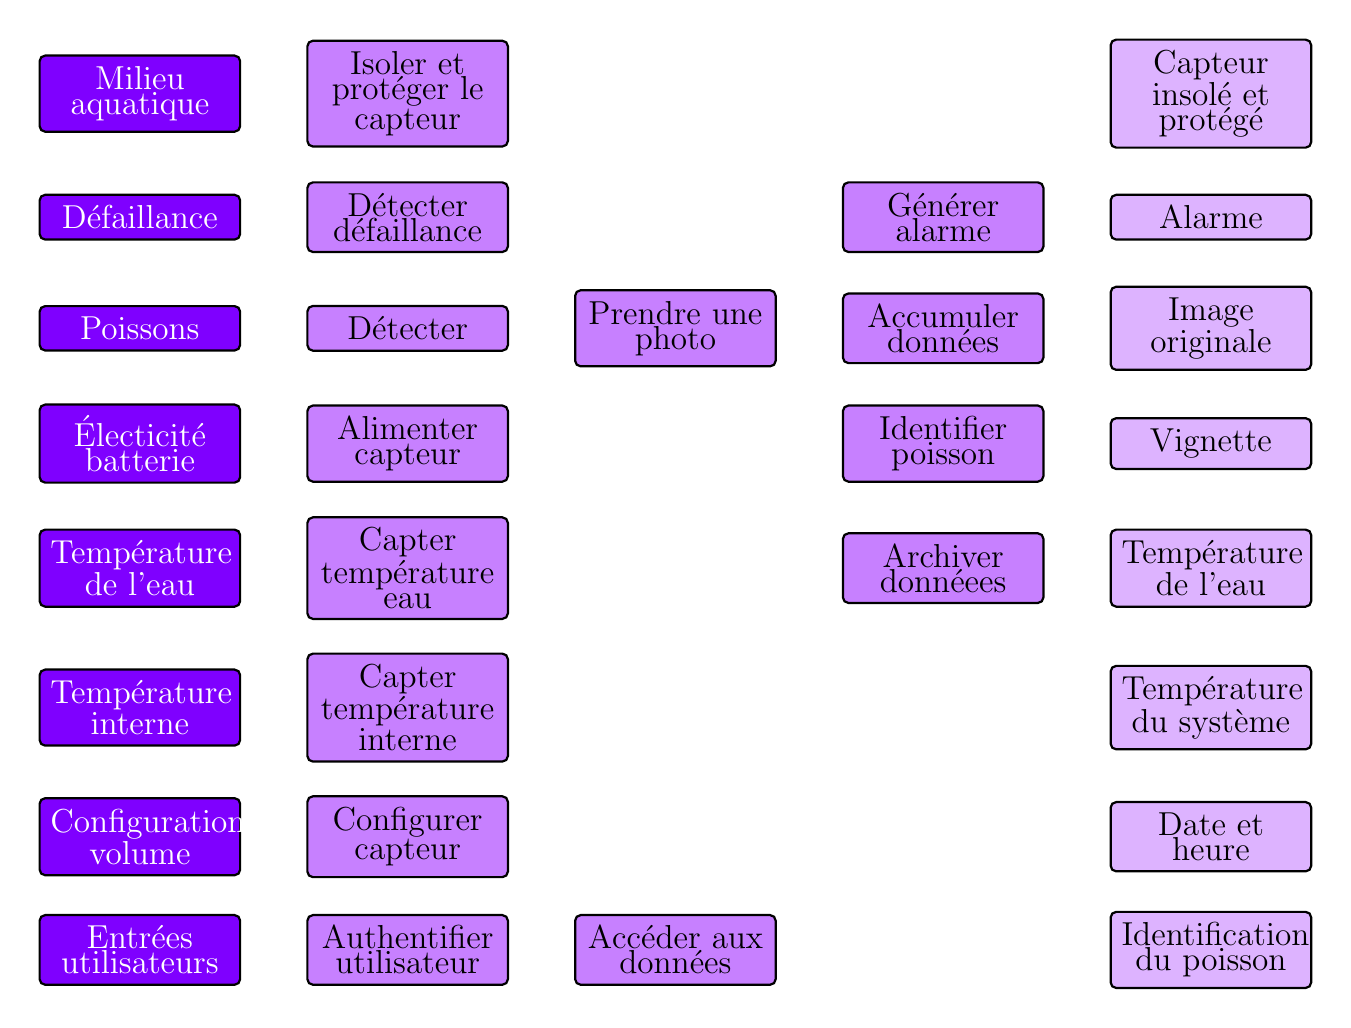
\begin{tikzpicture}[]
		\fontsize{12}{9} \selectfont
		% intrants
		\matrix[row sep=1em, column sep=2em] {
			% 1re ligne
			\node[intrant](forcutil){Milieu aquatique}; & \node[fonction](instcapt){Isoler et protéger le capteur}; & & & \node[extrant](captinst){Capteur insolé et protégé}; \\
			% 2me ligne
			\node[intrant](defailla){Défaillance}; & \node[fonction](detcdefa){Détecter défaillance}; & & \node[fonction](genralrm){Générer alarme}; & \node[extrant](alarme){Alarme}; \\
			% 3me ligne
			\node[intrant](poissons){Poissons}; & \node[fonction](detecteu){Détecter}; & \node[fonction](photo){Prendre une photo}; & \node[fonction](accudonn){Accumuler données}; & \node[extrant](imagorgi){Image originale}; \\
			% 4me ligne
			\node[intrant](elecbatt){Électicité batterie}; & \node[fonction](alimcapt){Alimenter capteur}; & & \node[fonction](idenpois){Identifier poisson}; & \node[extrant](vignette){Vignette}; \\
			% 5me ligne
			\node[intrant](tempreau){Température de l'eau}; & \node[fonction](captteau){Capter température eau}; & & \node[fonction](archdonn){Archiver donnéees}; & \node[extrant](tmpeauex){Température de l'eau}; \\
			% 6me ligne
			\node[intrant](tempintr){Température interne}; & \node[fonction](capttcpt){Capter température interne}; & & & \node[extrant](tmpintex){Température du système}; \\
			% 7me ligne
			\node[intrant](confvolm){Configuration volume}; & \node[fonction](confcapt){Configurer capteur}; & & & \node[extrant](dateheur){Date et heure}; \\
			% 8me ligne
			\node[intrant](entrutil){Entrées utilisateurs}; & \node[fonction](authutil){Authentifier utilisateur}; & \node[fonction](accedonn){Accéder aux données}; & & \node[extrant](idntpois){Identification du poisson}; \\
		};
		
		% Liens
		\lienhorz{forcutil}{instcapt}
		\lienhorz{defailla}{detcdefa}
		\lienhorz{poissons}{detecteu}
		\lienhorz{elecbatt}{alimcapt}
		\lienhorz{tempreau}{captteau}
		\lienhorz{tempintr}{capttcpt}
		\lienhorz{confvolm}{confcapt}
		\lienhorz{entrutil}{authutil}
		
		\lienhorz{detecteu}{photo}
		\lienhorz{detcdefa}{genralrm}
		\lienhorz{instcapt}{captinst}
		
		\lienhorz{authutil}{accedonn}
		
		\lienvtht{authutil}{confcapt}
		\lienvtbs{genralrm}{accudonn}
		\lienvtbs{accudonn}{idenpois}
		\lienvtbs{idenpois}{archdonn}
		
		\multiliens{genralrm,archdonn}{alarme}{1.5}
		\multiliens{photo,alimcapt,captteau,capttcpt,confcapt}{accudonn}{1}
		\liensparfaits{archdonn,accedonn}{imagorgi,vignette,tmpeauex,tmpintex,dateheur,idntpois}{0.5}{1}
	\end{tikzpicture}
	\caption{Diagramme fonctionnel}
	\label{f:caf_diag_fonc}
\end{figure}